\section{Network Management} \label{chap:nm} 

\par The topic of network management is very extensive, due to the several components that make up today's networks, and the vast amount of information that they
provide. It can be summed up as the operation and maintenance of network infrastructure so that the service it provides is not only "healthy", but also is operated
at a level that keeps costs down for service providers. 

\subsection {Requirements for management systems}

\par As the complexity of the networks, and network devices that compose them, grows bigger and bigger, the management systems should accommodate for the their
necessities. As such, the basic groups of requirements for management functions  defined in the ITU-T X 700 Recommendation \cite{noauthor_recommendation_1992}
are:

\begin {itemize}
    \item \textbf {Fault management} is the capability for detection, isolation and correction of abnormal operation in the system
    \item \textbf {Accounting management} provides ways to monitor the system resource utilization, and using this data to generate information about the costs that
        the operation of a certain resource will incur. This allows for optimizing the network utilization of resources, as it provides insights on how to
        plan the evolution of the network
    \item \textbf {Configuration management} is related to the maintenance and updates of hardware and software in the network, and the general setup of devices 
        that allow to start, maintain and terminate services 
    \item \textbf {Performance management} relates to monitor systems for the traffic utilization, response time, performance and logging histories. This allows to 
        maintain Service Level Agreements (SLA) between the service provider and the client, providing better services even in cases of unusual traffic.
    \item \textbf {Security management} enables setting up security policies in terms of access control to resources, private information protection, among others.
\end {itemize}

\par A network management system usually consists of a centralized station, and management agents running on the network devices. Using management protocols, the
agents can report to the station information about the its operational status, which includes information ranging from CPU load to bandwidth usage. Typically this
information can be retrieved by the controller polling the agents, or the agents sending information on their own, usually to inform status changes. Using this 
information, the network operator can get insight on the performance or possible errors of the devices that are monitored. In the next section, we explore one of the
most popular management protocols, SNMP.

\subsection {SNMP}

The Simple Network Management Protocol is an IETF defined protocol that allows for the interconnection of networking devices, and provide a structured way to
retrieve relevant information about these devices. As the name suggests, SNMP allows for a simplified approach to network monitoring, since it reduces the complexity
of the functions that the management agent needs to comply with, which bring several advantages, like reducing the costs for development of management tools;
provides a way to monitor, independently from different hardware providers the resources; and also supports freedom in extending the protocol in order to include
other aspects of network operation \cite{fedor_simple_1990}.
\par The architectural model of SNMP can be described in figure \ref{fig:snmp}.
    
\begin{figure} [!htbp]
    \centering
    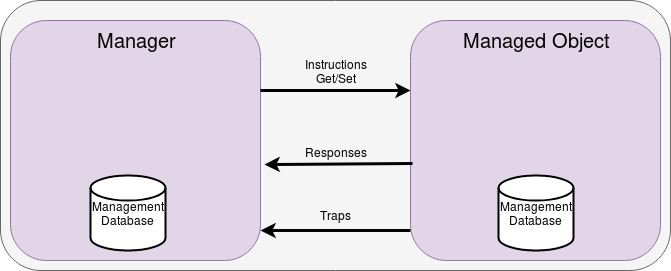
\includegraphics[width=.6\textwidth]{nm/snmp_arch}
    \caption{Architectural components of SNMP}
    \label{fig:snmp}
\end{figure}

The management database is one of the most important components of this system, because it serves as a reference to the entities that are managed in the SNMP
protocol. The formal name for this database is the MIB - Management Information Base \cite{rose_structure_1990}, and its composed of a collection of objects.

\par Each object has a name, syntax and encoding \cite{rose_management_1990}. The name of the object, more specifically, the \textit {Object Identifier (OID)}, is a
reference to the object itself. This name is usually a list of integers, and they serve to build a tree-like hierarchy. This structure allows for the organization 
of all objects in a logical pattern, as there is a parent node that contains references to their children, which provides different indexes for different objects. 
For human readability, there is usually an \textit {Object Descriptor}, to refer to the object type. 

\par The syntax defines the type of data structure in the object type; and the encoding describes how the object type is transmitted on the network. In the context
of this thesis, an important group is the interfaces group, as this exposes information about the interfaces present in a system. Its OID is the .3.6.1.2.1.2., 
and contains the number of interfaces in a system, and a table containing the counters related to the interface status, like the received unicast packets, the 
physical address, among others. The flexibility of the MIB allows for vendors to introduce their own databases into the MIB, while also remaining compatible 
with the standardized one.

\par Due to its permanence in the market, the protocol has suffered some large changes since its original design. SNMPv3 now supports important changes to the
original one, most notably in the security aspects, introducing strong authentication and encryption capabilities.

\par Despite it's dominance on network management products, SNMP features some bad characteristics that pose an obstacle for the widespread use in network
configuration and management, like \cite{schonwalder_overview_2003}: 

\begin {itemize}
    \item Incompleteness of the devices features
    \item SNMP access can sometimes crash systems, or return wrong data
    \item Unavailability of MIB modules, which forces users to use CLI's
    \item Poor performance 
    \item Security is difficult to handle
\end {itemize}

\subsection {Data Center Networks (DCN)}

\par The design of the network architecture is central to the data-center networks, as the placement for physical hosts and virtual machines allows for sharing the 
resources and create a logical hierarchy of network devices. The study on the design of DCN has resulted in the creation of typical DC topologies, like fat-tree
topologies (as seen in \ref{fig:fattree}), or others, including de Bruijn server only networks, or BCube switch heavy networks \cite{popa_cost_2010}. This approach
allows for the traffic characteristics, resource consumption and costs of the networking devices be monitored, so that causes for failure of this network are
understood and mitigated, and the entire DC can run on the most optimal way possible. The organization in the DCN also allows for traffic in the network being
resistant to failure scenarios, since there are multiple paths that can redirect packets to the correct destination, even if a link to a switch fails.

\begin{figure} [H]
    \centering
    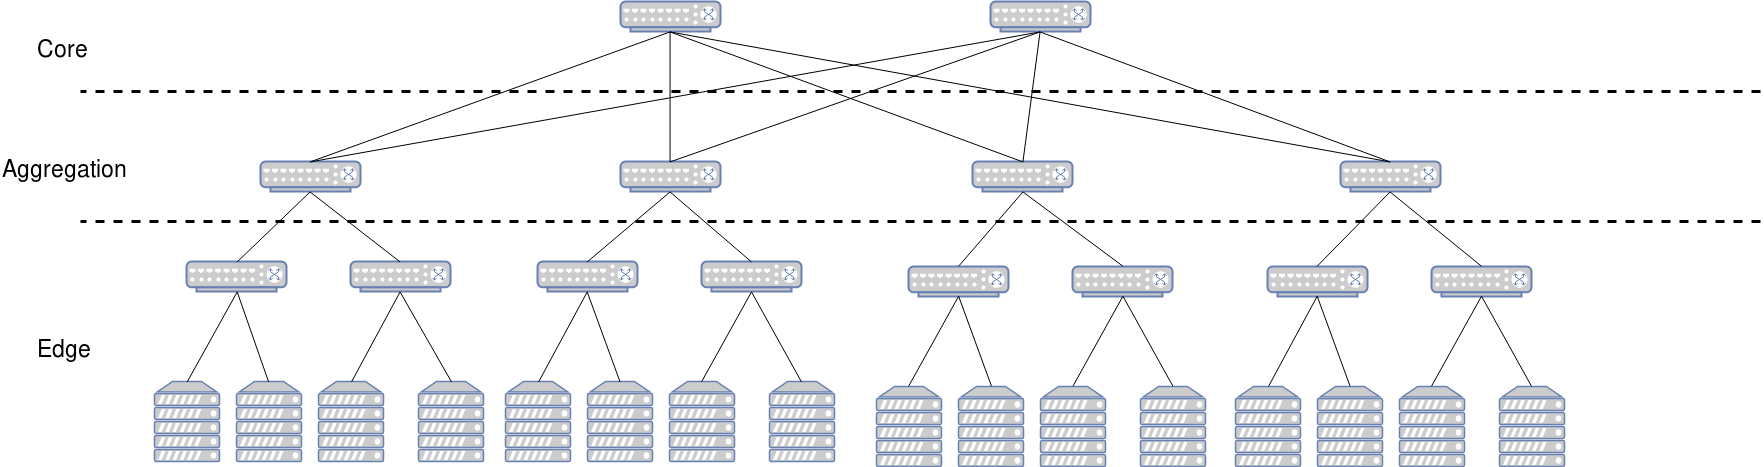
\includegraphics[width=1\textwidth]{nm/fattree}
    \caption{Visual representation of the fat tree topology commonly used in data centers}
    \label{fig:fattree}
\end{figure}

